\documentclass[11pt,a4paper,openany]{report}
\usepackage[T1]{fontenc}
\usepackage[utf8]{inputenc}
\usepackage{lmodern}
\usepackage{microtype}
\usepackage{amsmath,amssymb,amsthm,mathtools,bm}
\usepackage{booktabs,array,longtable,tabularx}
\usepackage{xcolor}
\usepackage[margin=22mm,headheight=23pt]{geometry}
\usepackage{enumitem}
\usepackage{fancyhdr}
\usepackage{fancyvrb}
\usepackage{graphicx}
\usepackage{url}
\usepackage{xurl}
\usepackage{hyperref}
\definecolor{finblue}{HTML}{1F5A99}
\definecolor{fingreen}{HTML}{19733A}
\definecolor{finorange}{HTML}{D55E00}
\definecolor{finred}{HTML}{A61B1B}
\definecolor{finviolet}{HTML}{6A3D9A}
\definecolor{fingray}{HTML}{4D4D4D}
\hypersetup{unicode=true,colorlinks=true,linkcolor=finblue,citecolor=fingreen,
urlcolor=finblue,pdftitle={FIN Local Research Checkpoint P475-P480-P484},
pdfauthor={Krzysztof Żuchowski},
pdfsubject={Dependency-minimal exact replay, algebraic elimination burden, and an adversarial phase-face audit},
pdfkeywords={FIN, quantum comb, Krawczyk operator, exact replay, algebraic elimination, complex optimal face}}
\pagestyle{fancy}\fancyhf{}
\fancyhead[L]{\small FIN Checkpoint P475/P480/P484}
\fancyhead[R]{\small Release 10.46}\fancyfoot[C]{\thepage}
\setlength{\parindent}{0pt}
\setlength{\parskip}{0.55em}
\setlist{nosep,leftmargin=2em}
\setcounter{tocdepth}{2}
\setcounter{secnumdepth}{3}
\emergencystretch=4em
\newcommand{\one}{\bm 1}
\newcommand{\C}{\mathbb C}
\newcommand{\R}{\mathbb R}
\newcommand{\Q}{\mathbb Q}
\newcommand{\statusProven}{\textcolor{fingreen}{[Proven]}}
\newcommand{\statusCAP}{\textcolor{fingreen}{[Computer-assisted proof]}}
\newcommand{\statusStrong}{\textcolor{finblue}{[Strong evidence]}}
\newcommand{\statusConditional}{\textcolor{finviolet}{[Conditional]}}
\newcommand{\statusOpen}{\textcolor{finorange}{[Open]}}
\newcommand{\statusRefuted}{\textcolor{finred}{[Refuted]}}

\begin{document}\hypersetup{pageanchor=false}
\begin{titlepage}\centering\vspace*{8mm}
{\Large\bfseries FIN Local Research --- Release 10.46\par}\vspace{10mm}
{\Huge\bfseries Checkpoint P475--P480--P484\par}\vspace{6mm}
{\Large Dependency-Minimal Exact Replay, Algebraic Elimination Burden,\par}
{\Large and an Adversarial Phase-Face Audit\par}\vspace{14mm}
{\Large Krzysztof \.Zuchowski\par}\vspace{2mm}
{\normalsize Independent Researcher --- Fractal Information Theory Project\par}
{\normalsize ORCID: 0009-0002-0909-3613\par}\vspace{8mm}
{\large 1 August 2026\par}
{\normalsize Publication --- Preprint; Version 1.0.0\par}
\vfill
\begin{minipage}{0.92\textwidth}\small
\textbf{Durable result.} The exact O180/O181 rational Krawczyk and positivity
certificate can now be independently replayed with the Python standard library
alone. A tampered certificate is rejected.

\medskip\textbf{Adversarial correction.} The proposed exact complex
phase-face theorem contains one unpaid implication: the invariant
three-dimensional axis has not been proved to satisfy the full causal
equal-endpoint constraint. An exact counterexample shows that odd dimension
and active Riccati congruence alone are insufficient. Full-cone nonuniqueness
therefore remains strong evidence, not a theorem.

\medskip\textbf{Algebraic boundary.} Exact lexicographic elimination did not
produce a polynomial for the optimum inside a 45-second, 3-GiB local envelope.
This is a method-specific resource result, not mathematical impossibility.

\medskip\textbf{License.} CC BY 4.0.
\end{minipage}\vfill
\end{titlepage}
\hypersetup{pageanchor=true}\pagenumbering{roman}
\chapter*{Publication statement}\addcontentsline{toc}{chapter}{Publication statement}
This monograph reports local analytical and computational Programs P475,
P480, and P484. It uses no network, Firecrawl, external AI, external audit,
remote computation, laboratory record, or empirical physical evidence.
\tableofcontents\clearpage\pagenumbering{arabic}

\chapter{Executive summary}

This checkpoint follows the exact O167 attainment certificate of P473 and its
uniform local continuation in P483. It was designed to do three different
jobs: reduce verifier dependencies, attack the algebraic value directly, and
attempt to turn the P474 complex-flat-direction evidence into a theorem.

\begin{enumerate}
\item \textbf{P480 --- \statusCAP{} replayed.} A serialized rational document
contains the 13 equations, all 169 Jacobian entries, the rational root box,
algebraic sine enclosures, preconditioner, center matrices, and positivity
bounds. A new checker using only the Python standard library recomputes exact
interval Krawczyk inclusion and exact Sylvester payments. It rejects a zeroed
preconditioner in an adversarial test.

\item \textbf{P484 --- \statusStrong{}; exact step open.} Nine exact symbolic
identities yield a clean three-plus-three parity reduction. Six numerical
tangent equations agree through 80 displayed digits, and residuals are at
machine precision. The attempted analytic proof nevertheless needs the fixed
covector of a metric rotation to lie in a particular causal plane. An exact
rational counterexample proves that odd-dimensional metric orthogonality and
the active Riccati equations do not imply this. The repository-specific
shared-entry and standard-sector identities may still imply it, but that
claim has not been certified. The exact phase face and full-cone
nonuniqueness remain open.

\item \textbf{P475 --- \statusOpen{}; resource-bounded no-go.} All sine
coefficients reduce to the degree-four field \(\Q(\sin(\pi/8))\). The exact
Riccati system is cubic over that field and affine in the three normalizer
coordinates. A bounded exact lexicographic Gr\"obner attempt returned no
univariate relation for the value \(L\) before its hard resource stop. This
does not imply that no minimal polynomial exists.
\end{enumerate}

The strongest positive result is the dependency-minimal P480 replay. The
strongest falsification result is the P484 correction: a beautiful structural
argument is not promoted beyond the exact implication actually paid by the
artifacts.

The new objects are O185 Conditional Odd-Dimensional Complex Comb Phase Face,
O186 Dependency-Minimal Exact O181 Replay Certificate, and O187
Resource-Bounded Algebraic Elimination Burden Certificate.

\chapter{Confidence convention and state transition}

\begin{center}\small
\begin{longtable}{@{}p{0.39\textwidth}p{0.47\textwidth}@{}}
\toprule
\textbf{Label} & \textbf{Meaning}\\ \midrule\endhead
\statusProven{} & Exact analytic or finite symbolic consequence of declared premises\\
\statusCAP{} & Finite rational or outward-interval certificate with auditable artifacts\\
\statusStrong{} & Reproducible numerical evidence missing one exact certificate\\
\statusConditional{} & Exact implication after an explicitly named open premise\\
\statusOpen{} & Current local artifacts do not decide the proposition\\
\statusRefuted{} & A necessary implication fails by exact counterexample\\
\bottomrule
\end{longtable}
\end{center}

\begin{center}\small
\begin{longtable}{@{}p{0.31\textwidth}p{0.22\textwidth}p{0.32\textwidth}@{}}
\toprule
\textbf{Lane} & \textbf{Status} & \textbf{Boundary}\\ \midrule\endhead
Nominal O181 root and O167 attainment & \statusCAP{} & Declared reduced ordered three-slot comb\\
P483 parameter tube & \statusCAP{} & Tiny dimensionless rectangle; one local box\\
Dependency-minimal replay & \statusCAP{} replayed & Finite root and positivity part only\\
Full complex optimizer uniqueness & \statusOpen{} & Strong evidence against; exact causal-axis step missing\\
Minimal polynomial of \(L\) & \statusOpen{} & Blind exact lexicographic route exceeded declared resources\\
Lean formalization & Source only & No local Lean toolchain; not machine checked\\
Selector / QW-2191 & \statusOpen{} & No non-premise strict source\\
Dimensional source & Missing & No time, length, action, mass, or energy unit\\
Physical realization & Externally blocked & No apparatus, calibration, custody, or laboratory record\\
Legacy--strict bridge and role transfer & Incomplete & No silent substitution or inherited role\\
\bottomrule
\end{longtable}
\end{center}

\chapter{Inherited exact operator problem}

For the supplied compressed Hermitian process difference \(\Delta\), the
declared ordered three-slot primal optimizes
\[
 \frac12\operatorname{Tr}[\Delta(T_+-T_-)]
\]
over positive tester effects with the nested comb normalization. At a fixed
positive normalizer \(N=T_++T_-\), the inner value is
\[
 F(N)=\frac12\left\|N^{1/2}\Delta N^{1/2}\right\|_1.
\]

P473 certified an exact positive root of the structured Riccati system
\[
 X_3NX_3=\frac14\Delta N\Delta                                     \tag{3.1}
\]
inside a rational 13-dimensional box of radius \(3\times10^{-14}\).
The block pattern pays all lower dual equalities; the positive support theorem
and trace telescope then give exact primal--dual attainment. P483 proved the
same conclusion uniformly for
\[
 |q-4/5|\le3\times10^{-9},\qquad
 |\theta-\pi/8|\le3\times10^{-9}.
\]

These are local root results in a real polynomial chart. They do not establish
uniqueness in the complete complex causal cone.

\chapter{P480: dependency-minimal exact replay}

\section{Question and success criterion}

The exact numerical certificate previously depended on a builder using
NumPy, SciPy, and SymPy. P480 asks whether a verifier can recompute the finite
proof using only exact rational arithmetic available in a default Python
installation. Success requires recomputation rather than trust in stored
Boolean fields.

\section{Certificate schema}

The JSON certificate serializes:
\begin{itemize}
\item 13 rational polynomial equations as monomial/exponent lists;
\item all \(13\times13=169\) rational Jacobian polynomials;
\item the 13-coordinate rational center and radius
      \(r=3\times10^{-14}\);
\item exact rational enclosures for \(\sin(k\pi/8)\), \(k=1,2,3\);
\item a rational approximate inverse \(R\);
\item rational center matrices \(N_c\) and \(X_{3,c}\);
\item declared entry Lipschitz constants and a Sylvester margin.
\end{itemize}

The checker imports only \texttt{fractions}, \texttt{json},
\texttt{pathlib}, \texttt{sys}, \texttt{typing}, and
\texttt{\_\_future\_\_}. An abstract-syntax regression test enforces this
boundary.

\section{Exact Krawczyk computation}

Let \(F:\R^{13}\to\R^{13}\), let
\(X=x_c+[-r,r]^{13}\), and let \(J(X)\) be the exact interval Jacobian.
The verifier constructs
\[
 \mathcal K(X)=x_c-RF(x_c)+(I-RJ(X))(X-x_c).                         \tag{4.1}
\]
All interval endpoints are \texttt{Fraction} objects. Strict coordinatewise
inclusion
\[
 \mathcal K(X)\subset\operatorname{int}X
\]
is recomputed. The diagnostics are
\begin{align*}
\text{minimum inward margin}&\approx1.8189522605\times10^{-14},\\
\text{maximum contraction row sum}&\approx6.8847446957\times10^{-10},\\
\text{maximum point-residual radius}&\approx6.6004906310\times10^{-17}.
\end{align*}

The exact value interval is
\[
 \frac{5233281002710117}{10^{16}}
 \le L\le
 \frac{5233281002710717}{10^{16}},
 \qquad |I_L|=\frac3{5\times10^{13}}.                              \tag{4.2}
\]

\section{Exact positivity payments}

The checker performs exact fraction Gaussian elimination on every leading
principal minor of
\[
 N_c-\frac1{100}I,
 \qquad X_{3,c}-\frac1{100}I.
\]
All are positive. Paying the full box perturbation gives
\[
 N\succeq\frac{24999999997}{2500000000000}I,
 \qquad
 X_3\succeq\frac{124999999997}{12500000000000}I.                   \tag{4.3}
\]

\section{Adversarial rejection}

The test suite replaces the rational preconditioner by the zero matrix. Then
(4.1) loses strict inward inclusion, and the checker returns failure. This
demonstrates that the verifier does not merely echo a precomputed acceptance
field.

\section{O186 interface}

O186 is the \emph{Dependency-Minimal Exact O181 Replay Certificate}. Its
domain is a finite rational JSON document; its codomain is an accept/reject
decision with exact diagnostic margins. Removing monomials or the Jacobian
prevents recomputation. Removing strict inclusion destroys the uniqueness
certificate. Removing positivity payments leaves the operator root
inadmissible for the attainment theorem.

O186 checks the finite root and positivity component. The
Riccati-to-support and trace-telescope implications remain analytic theorems;
O186 is not a physical measurement validator.

\chapter{P484: adversarial phase-face audit}

\section{Candidate complex tangent}

Write \(\Delta=iK\), where \(K\) is real skew. An imaginary Hermitian
normalizer displacement has the form
\[
 N(t)=N+i tQ,\qquad Q^T=-Q.
\]
Because (3.1) is linear in \(N\), a flat affine direction must satisfy
\[
 X_3QX_3+\frac14KQK=0.                                             \tag{5.1}
\]

The P474 finite contact matrix had rank 127 in 128 real coordinates. An
independent imaginary-causal tangent map had rank six in seven coordinates.
Both calculations indicated one candidate direction, but neither was exact.

\section{Exact parity reduction}

An exact swap/complement basis gives the active sector
\[
 N=N_0\oplus N_0,qquad
 X_3=X_+\oplus X_-,qquad
 K=\begin{pmatrix}0&C\\-C^T&0\end{pmatrix}.                       \tag{5.2}
\]
The executable proof checks nine exact representation identities: basis
orthonormality, vanishing parity off-blocks, equality of the two normalizer
blocks, the skew relation between the two \(K\) cross blocks, and both
standard-sector formulas.

The positive Riccati congruences imply
\[
 X_- = \frac14 C^T X_+^{-1} C,                                    \tag{5.3}
\]
so with
\[
 B=\frac12X_-^{-1}C^T
\]
one obtains \(BN_0B^T=N_0\). Conditional on \(\det B=1\), odd dimension
gives a fixed covector and an invariant skew form. If this covector lies in
the equal-endpoint causal plane, it lifts to a nonzero exact solution of
(5.1). Exact positivity would then produce a nonzero constant-value segment.

\section{The missing implication}

The last sentence contains a genuine additional premise. Odd dimension does
not force the fixed covector into the required causal plane.

Take
\[
 N_0=X_+=X_-=I_3,\qquad v=(1,0,2)^T,
\]
and define the rational half-turn
\[
 B=\frac{2vv^T}{v^Tv}-I_3
 =\begin{pmatrix}
 -3/5&0&4/5\\0&-1&0\\4/5&0&3/5
 \end{pmatrix},
 \qquad C=2B^T.                                                     \tag{5.4}
\]
Exact symbolic arithmetic gives
\[
 BB^T=I_3,\quad\det B=1,\quad B^Tv=v,
\]
and
\[
 I_3-CC^T/4=0,\qquad I_3-C^TC/4=0.                                \tag{5.5}
\]
Thus both active Riccati blocks and orientation-preserving metric
orthogonality hold, but \(v_1\ne v_3\). The claimed automatic causal-axis
implication is \statusRefuted{}.

This counterexample does not satisfy all additional FIN shared-entry and
standard-sector constraints. It therefore does not refute the specific P473
candidate. It proves exactly why those additional equations require a new
identity or certificate.

\section{Evidence that survives}

At the P473 branch the computed map has
\[
 \det B\approx1,qquad
 \sigma(B)=\{1,0.2704387824\pm0.9627371734i\}.
\]
Its fixed covector, normalized by the first entry, is
\[
 (1,0.02106502319,0.9999999999999978)^T,
\]
with equal-endpoint residual \(2.22\times10^{-15}\). Six tangent equations
return the common displayed value
\[
 \rho\approx0.02979044149309996478959538442548707608969921737694\ldots
\]
through 80 digits. A 180-digit rerun resolves differences near
\(10^{-102}\), at the finite nonlinear-solve tolerance. The tangent residual
is \(6.65\times10^{-16}\).

These figures are strong numerical evidence. They cannot establish an exact
zero or an exact affine face.

\begin{figure}[htbp]
\centering
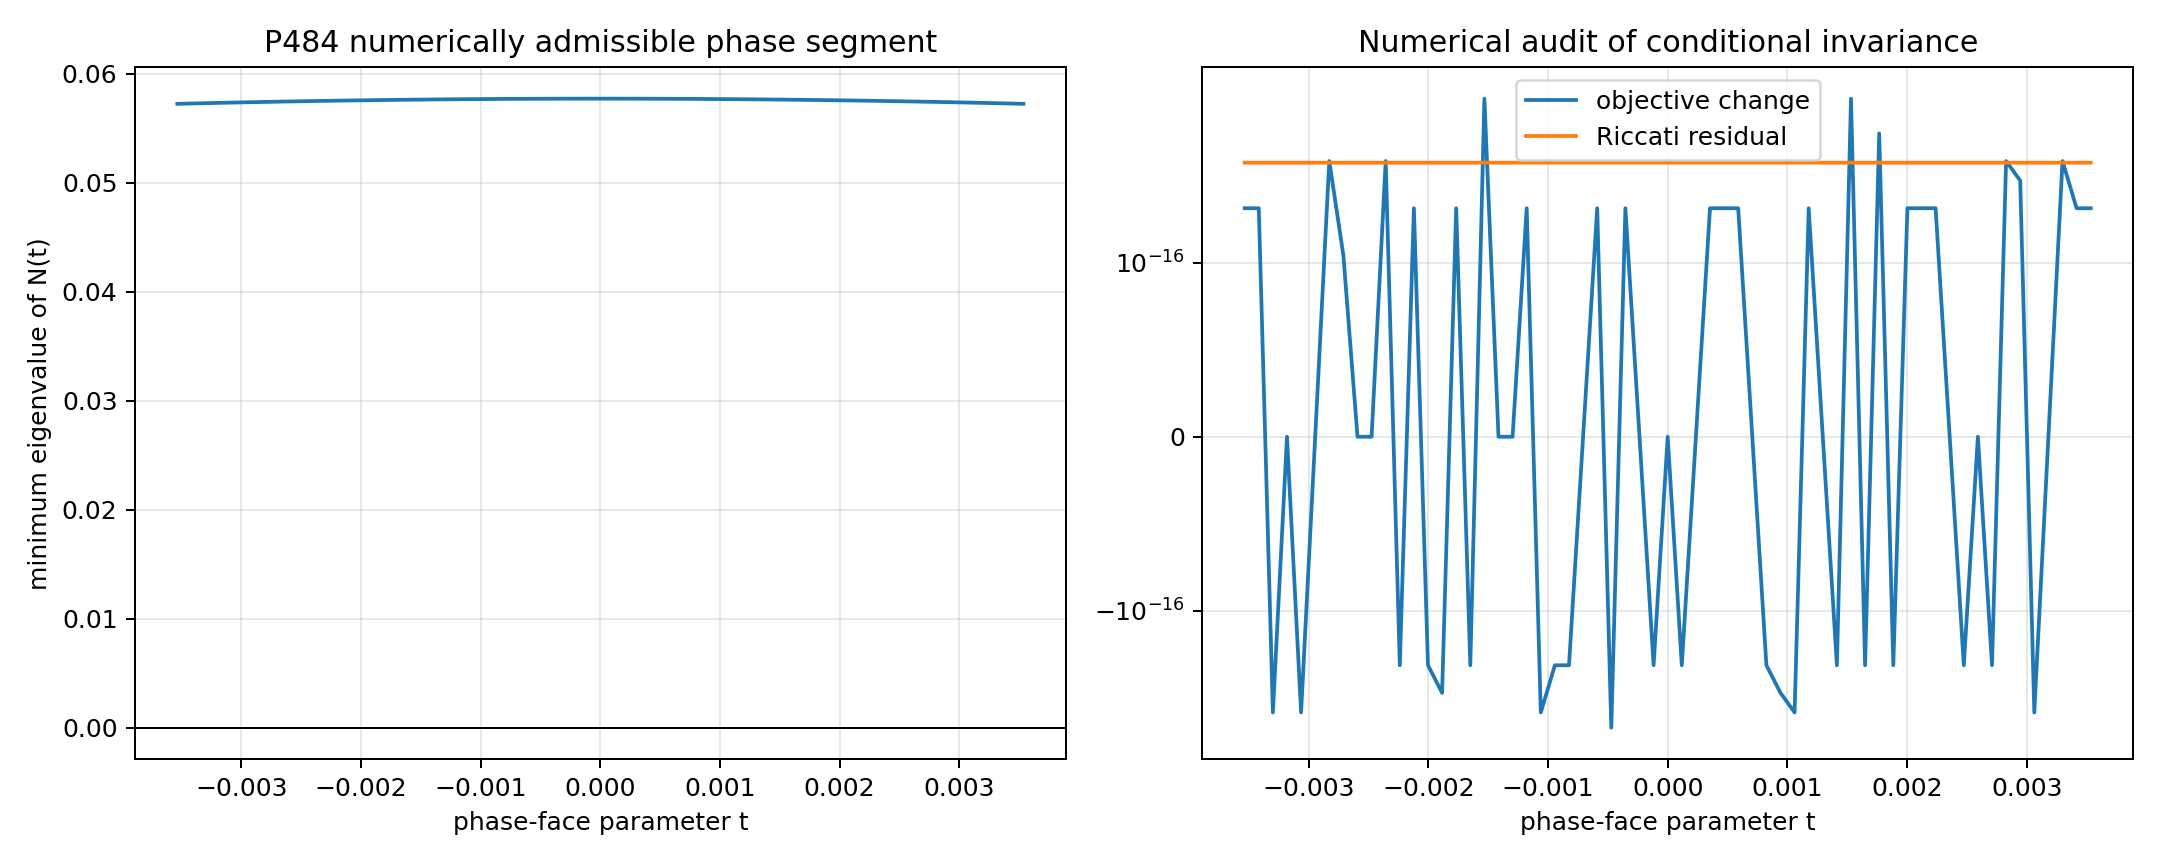
\includegraphics[width=0.96\textwidth]{FIN_Program_484_Figures/p484_exact_complex_phase_face.png}
\caption{Numerical audit of the conditional P484 phase segment. Positivity
and constant objective are sampled, while exact causality of the tangent
remains the named proof obligation.}
\end{figure}

\section{Corrected theorem status}

The representation reduction and counterexample (5.4)--(5.5) are
\statusProven{}. The existence of an exact nonzero causal tangent at the exact
P473 root is \statusStrong{} with one explicit missing identity. Full-cone
optimizer uniqueness is neither proved nor refuted. O185 is therefore a
\emph{Conditional Odd-Dimensional Complex Comb Phase Face}.

\chapter{P475: resource-bounded algebraic elimination}

\section{Exact algebraic coefficient field}

Let \(\alpha=\sin(\pi/8)\). Then
\[
 8\alpha^4-8\alpha^2+1=0,                                        \tag{6.1}
\]
and
\[
 \sin(\pi/4)=1-2\alpha^2,
 \qquad
 \sin(3\pi/8)=3\alpha-4\alpha^3.                                \tag{6.2}
\]
The extension degree is four. Indeed, for \(y=2\alpha\),
\(y^4-4y^2+2\) is Eisenstein at 2.

After (6.2), the exact problem contains 13 equations in 13 operator
coordinates over \(\Q(\alpha)\). Each equation has operator-coordinate degree
at most three. Representing \(\alpha\) as a fourteenth rational-elimination
variable raises the largest total degree to seven. The largest equation has
29 monomials, and the full list has 262 monomial occurrences.

\section{Affine normalizer structure}

Every Riccati equation is affine in \(A,B,u\), the three normalizer
coordinates. A floating pivot scout selects equation rows 5, 10, and 11. The
corresponding exact determinant is a nonzero polynomial of total degree 10
with 409 terms; at the floating root its absolute value is approximately
\(0.02238991248\).

This is a route proposal, not yet a certified elimination: nonzero as a
polynomial and nonzero at a floating locator do not prove nonvanishing over
the exact root box.

\section{Declared elimination envelope}

The exact worker adds (6.1) and requests a lexicographic Gr\"obner basis in
14 variables, ordering \(L\) last. It is restricted to
\begin{itemize}
\item 40 seconds CPU time;
\item 45 seconds wall time;
\item 3 GiB address space;
\item SymPy 1.12 on the local Intel i3-10110U / 16 GB host;
\item no network, external CAS, or remote computation.
\end{itemize}

The parent terminated the worker after \(45.0778\) seconds. No univariate
relation in \(L\) was returned. The crude number
\[
 3^{13}=1,594,323
\]
is only a projective cubic B\'ezout bound over \(\Q(\alpha)\); it is not a
root count and does not incorporate positivity or local branch admission.

\section{Interpretation of the no-go}

P475 proves the exact coefficient-field reduction, polynomial inventory,
affine normalizer dependence, and faithful resource stop. It does not prove
transcendence, nonexistence of a minimal polynomial, ideal dimension,
algebraic degree, or global solution count.

O187 is the \emph{Resource-Bounded Algebraic Elimination Burden
Certificate}. It can be falsified constructively by a future modular,
resultant, homotopy-assisted, or structure-aware exact workflow that returns
and verifies a relation under a comparable envelope.

\chapter{Falsification ledger}

\begin{center}\small
\begin{longtable}{@{}p{0.22\textwidth}p{0.26\textwidth}p{0.29\textwidth}@{}}
\toprule
\textbf{Candidate claim} & \textbf{Attack} & \textbf{Verdict}\\ \midrule\endhead
P480 merely trusts a stored verdict & Zero every preconditioner entry & Rejected; strict inclusion fails\\
P480 needs the scientific Python stack to verify & Audit imports and replay from JSON & Refuted; standard library suffices\\
Odd dimension automatically supplies the causal P484 tangent & Exact rational half-turn with axis \((1,0,2)\) & Refuted for active Riccati/metric premises alone\\
The P473 phase candidate is merely numerical noise & Independent contact and tangent maps; precision escalation & Strong evidence against noise, but exact zero still open\\
Direct exact lexicographic elimination is cheap locally & Hard-bounded 14-variable run & Refuted only inside the declared implementation/resource envelope\\
P475 proves no minimal polynomial exists & Logical boundary audit & Refuted; no such conclusion follows from timeout\\
\bottomrule
\end{longtable}
\end{center}

\chapter{Kernel, selector, dimensional, and physical audit}

The binding split remains
\[
 K_{\mathrm{legacy,ont}}(d)=
 \frac{\alpha_{\mathrm{geo}}\cos(\omega d+\phi)}
      {1+\beta_{\mathrm{tors}}d},
 \qquad
 K_{\mathrm{strict,gate}}(d)=
 \frac{\cos(\omega d+\phi)}{1+\beta d^\eta}.                      \tag{8.1}
\]

Programs P475/P480/P484 analyze a supplied downstream finite channel. They
derive neither member of (8.1), complete no bridge, and transfer no legacy
electroweak, electromagnetic, gravitational-hierarchy, or other physical
role.

QW-2191 remains open. A complex affine degree of freedom, even if P485 later
proves it exact, is not automatically a selector, orientation source, or
observable. It supplies no clock, preparation, instrument, environment,
apparatus, observer, or measurement record.

All quantities remain dimensionless. Mathematical duality
\[
 U_t=e^{-itA},\qquad P_t=e^{-tA}
\]
does not generate a calibrated physical time or laboratory implementation.
No synthetic datum is treated as empirical evidence.

The internal ontology remains
\[
 \text{nadsoliton}\longrightarrow\text{light}\longrightarrow
 \text{matter}\longrightarrow\text{emergent observer},
\]
with no informational layer beneath the nadsoliton. This checkpoint neither
falsifies nor physically validates that ontology.

\chapter{Recommended next programs}

\begin{center}\scriptsize
\begin{longtable}{@{}r p{0.10\textwidth}p{0.55\textwidth}r@{}}
\toprule
\textbf{Rank}&\textbf{Program}&\textbf{Decisive local question}&\textbf{Chance}\\ \midrule\endhead
1&P485&Exact ideal identity or certified counterexample for the P473 shared-entry/standard-sector causal-axis implication&55\%\\
2&P486&Certify \(\det C>0\), \(\det B=1\), and all orientation premises uniformly on the P473 box&80\%\\
3&P487&Eliminate \(A,B,u\) through a certified pivot and try a ten-variable structure-aware resultant/Gr\"obner route&50\%\\
4&P488&Finite-field Gr\"obner scouting plus Chinese-remainder reconstruction of a candidate polynomial for \(L\)&35\%\\
5&P489&Conditional on P485, certify persistence of the complex phase face on a nonzero P483 sub-tube&30\%\\
6&P490&Build an independent second P480 implementation and differential-test exact verdicts&75\%\\
7&P491&Bound the local algebraic degree of O181 without computing the full minimal polynomial&45\%\\
8&P492&Certify the complete complex contact-face dimension or a transverse rank lower bound&40\%\\
9&P493&Interval-certified sensitivities \(dL/dq\) and \(dL/d\theta\)&75\%\\
10&P494&Grow the P483 parameter cover until a certified inclusion, positivity, or conditioning boundary&70\%\\
11&P495&Seek a bounded four-slot support theorem or a counterexample from the exact two-/three-slot reductions&30\%\\
12&P496&Formalize the minimum operational data needed to make O167 observable and prove the local empirical boundary&85\%\\
13&P497&Audit which O167 inputs are kernel-split robust and which require a typed completion atom&70\%\\
\bottomrule
\end{longtable}
\end{center}

The selected next bounded batch is
\[
 \boxed{P485\longrightarrow P486\longrightarrow P487}.            \tag{9.1}
\]
P485 decides whether P474/P484 becomes an exact nonuniqueness theorem or
remains numerical evidence. P486 pays the orientation premise separately.
P487 exploits P475's affine structure instead of repeating blind full
lexicographic elimination.

\chapter{Reproducibility and artifact hand-off}

\section{Restart commands}

\begin{Verbatim}[fontsize=\small]
MPLCONFIGDIR=/tmp/matplotlib python3 fin_program_484.py
MPLCONFIGDIR=/tmp/matplotlib python3 fin_program_480_build_certificate.py
python3 fin_program_480_standalone_checker.py
MPLCONFIGDIR=/tmp/matplotlib python3 fin_program_475.py
python3 -m unittest -v test_fin_programs_480_484.py
\end{Verbatim}

P475 intentionally consumes up to 45 seconds and is expected to report the
bounded timeout on the present host. P480 replay itself requires no scientific
Python dependency.

\section{Primary artifacts}

\begin{itemize}
\item \path{FIN_Local_Research_Checkpoint_P475_P480_P484_EN.md}
\item \path{FIN_Local_Research_Checkpoint_P475_P480_P484_EN.tex}
\item \path{FIN_Local_Research_Checkpoint_P475_P480_P484_EN.pdf}
\item \path{FIN_Local_Research_Checkpoint_P475_P480_P484_State.json}
\item \path{FIN_Program_475_Results.json}
\item \path{FIN_Program_475_Algebraic_Inventory.csv}
\item \path{fin_program_475.py}
\item \path{fin_program_475_elimination_worker.py}
\item \path{FIN_Program_480_Standalone_Certificate.json}
\item \path{FIN_Program_480_Standalone_Check_Result.json}
\item \path{fin_program_480_build_certificate.py}
\item \path{fin_program_480_standalone_checker.py}
\item \path{FIN_Program_484_Results.json}
\item \path{FIN_Program_484_Symmetry_Phase_Face.csv}
\item \path{FIN_Program_484_Phase_Face_Witness.npz}
\item \path{FIN_Program_484_Figures/p484_exact_complex_phase_face.png}
\item \path{fin_program_484.py}
\item \path{test_fin_programs_480_484.py}
\item \path{RELEASE_10_46_PROGRAMS_475_480_484.md}
\item \path{FIN_Checkpoint_P475_P480_P484_AGENTS_Guardrail.txt}
\item \path{FIN_PROGRAMS_475_480_484_RELEASE_MANIFEST.sha256}
\end{itemize}

\chapter{Conclusion}

Release 10.46 improves rigor in two opposite but complementary ways. It makes
the exact O181 certificate substantially easier to audit, and it withdraws an
exact phase-face conclusion that the current artifacts do not yet prove.

The mathematical frontier is now sharp. Either the additional FIN
shared-entry and standard-sector equations force the observed causal axis
exactly, or the near-perfect numerical phase direction is only approximate.
P485 can ask this as a finite, falsifiable local problem. No cosmological or
physical interpretation is needed to state or decide it.

No selector closure, dimensional source, laboratory validation,
legacy-to-strict completion, role transfer, \(L_{\mathrm{total}}\), Standard
Model, gravity, or Theory-of-Everything closure is claimed.

\end{document}
